
\documentclass[12 pt]{article}  %

\usepackage{verbatim}
\usepackage{graphicx}
\usepackage[hypertexnames=true,colorlinks=true,breaklinks]{hyperref}
\usepackage[margin=0.5in]{geometry}

\title{New Latent Variables Estimation Method}

\author{Joaquin Rapela}

\begin{document}

\maketitle

\listoffigures

\begin{figure}
    \begin{center}
        \href{../figures/latent1.html}{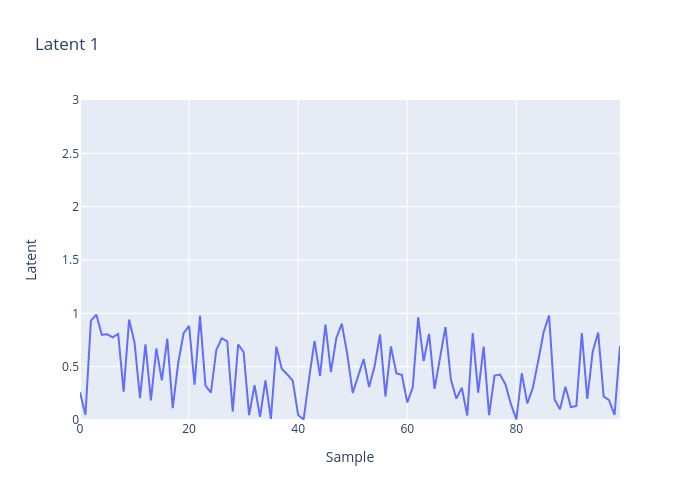
\includegraphics[width=7in]{../figures/latent1.png}}
        \caption{Estimated latent 1}
        \label{fig:latent1}
    \end{center}
\end{figure}

\begin{figure}
    \begin{center}
        \href{../figures/latent2.html}{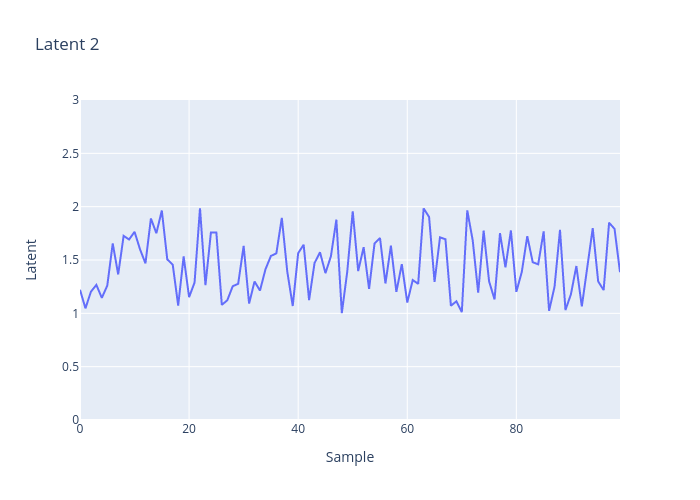
\includegraphics[width=7in]{../figures/latent2.png}}
        \caption{Estimated latent 2}
        \label{fig:latent2}
    \end{center}
\end{figure}

\begin{figure}
    \begin{center}
        \href{../figures/latent3.html}{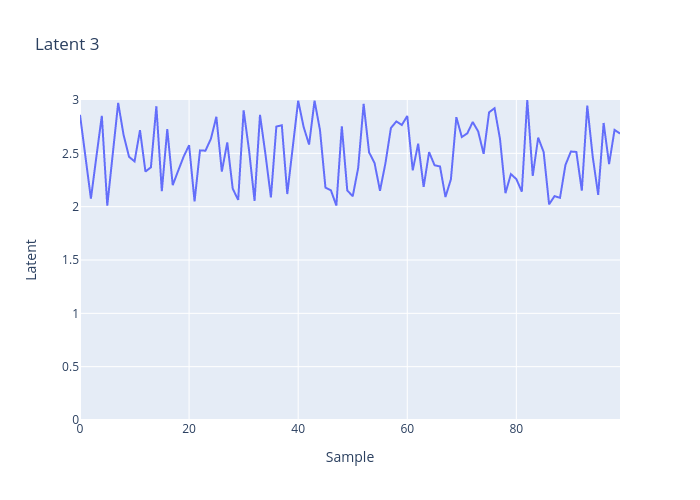
\includegraphics[width=7in]{../figures/latent3.png}}
        \caption{Estimated latent 3}
        \label{fig:latent3}
    \end{center}
\end{figure}

\end{document}
